\batchmode
\documentclass[twoside]{article}

% Packages required by doxygen
\usepackage{fixltx2e}
\usepackage{calc}
\usepackage{doxygen}
\usepackage[export]{adjustbox} % also loads graphicx
\usepackage{graphicx}
\usepackage[utf8]{inputenc}
\usepackage{makeidx}
\usepackage{multicol}
\usepackage{multirow}
\PassOptionsToPackage{warn}{textcomp}
\usepackage{textcomp}
\usepackage[nointegrals]{wasysym}
\usepackage[table]{xcolor}

% Font selection
\usepackage[T1]{fontenc}
\usepackage[scaled=.90]{helvet}
\usepackage{courier}
\usepackage{amssymb}
\usepackage{sectsty}
\renewcommand{\familydefault}{\sfdefault}
\allsectionsfont{%
  \fontseries{bc}\selectfont%
  \color{darkgray}%
}
\renewcommand{\DoxyLabelFont}{%
  \fontseries{bc}\selectfont%
  \color{darkgray}%
}
\newcommand{\+}{\discretionary{\mbox{\scriptsize$\hookleftarrow$}}{}{}}

% Page & text layout
\usepackage{geometry}
\geometry{%
  letterpaper,%
  top=2.5cm,%
  bottom=2.5cm,%
  left=2.5cm,%
  right=2.5cm%
}
\tolerance=750
\hfuzz=15pt
\hbadness=750
\setlength{\emergencystretch}{15pt}
\setlength{\parindent}{0cm}
\setlength{\parskip}{3ex plus 2ex minus 2ex}
\makeatletter
\renewcommand{\paragraph}{%
  \@startsection{paragraph}{4}{0ex}{-1.0ex}{1.0ex}{%
    \normalfont\normalsize\bfseries\SS@parafont%
  }%
}
\renewcommand{\subparagraph}{%
  \@startsection{subparagraph}{5}{0ex}{-1.0ex}{1.0ex}{%
    \normalfont\normalsize\bfseries\SS@subparafont%
  }%
}
\makeatother

% Headers & footers
\usepackage{fancyhdr}
\pagestyle{fancyplain}
\fancyhead[LE]{\fancyplain{}{\bfseries\thepage}}
\fancyhead[CE]{\fancyplain{}{}}
\fancyhead[RE]{\fancyplain{}{\bfseries\leftmark}}
\fancyhead[LO]{\fancyplain{}{\bfseries\rightmark}}
\fancyhead[CO]{\fancyplain{}{}}
\fancyhead[RO]{\fancyplain{}{\bfseries\thepage}}
\fancyfoot[LE]{\fancyplain{}{}}
\fancyfoot[CE]{\fancyplain{}{}}
\fancyfoot[RE]{\fancyplain{}{\bfseries\scriptsize Generated by Doxygen }}
\fancyfoot[LO]{\fancyplain{}{\bfseries\scriptsize Generated by Doxygen }}
\fancyfoot[CO]{\fancyplain{}{}}
\fancyfoot[RO]{\fancyplain{}{}}
\renewcommand{\footrulewidth}{0.4pt}
\renewcommand{\sectionmark}[1]{%
  \markright{\thesection\ #1}%
}

% Indices & bibliography
\usepackage{natbib}
\usepackage[titles]{tocloft}
\setcounter{tocdepth}{3}
\setcounter{secnumdepth}{5}
\makeindex

% Hyperlinks (required, but should be loaded last)
\usepackage{ifpdf}
\ifpdf
  \usepackage[pdftex,pagebackref=true]{hyperref}
\else
  \usepackage[ps2pdf,pagebackref=true]{hyperref}
\fi
\hypersetup{%
  colorlinks=true,%
  linkcolor=blue,%
  citecolor=blue,%
  unicode%
}

% Custom commands
\newcommand{\clearemptydoublepage}{%
  \newpage{\pagestyle{empty}\cleardoublepage}%
}

\usepackage{caption}
\captionsetup{labelsep=space,justification=centering,font={bf},singlelinecheck=off,skip=4pt,position=top}

%===== C O N T E N T S =====

\begin{document}

% Titlepage & ToC
\hypersetup{pageanchor=false,
             bookmarksnumbered=true,
             pdfencoding=unicode
            }
\pagenumbering{roman}
\begin{titlepage}
\vspace*{7cm}
\begin{center}%
{\Large Backtrace\+Exception }\\
\vspace*{1cm}
{\large Generated by Doxygen 1.8.11}\\
\end{center}
\end{titlepage}
\tableofcontents
\pagenumbering{arabic}
\hypersetup{pageanchor=true}

%--- Begin generated contents ---
\section{Main Page}
\label{index}\hypertarget{index}{}Backtrace\-Exception is a C++ exception type that produces a backtrace when thrown. It can capture this backtrace with several methods and the backtrace can be disabled. The goal is for the library to work on both Linux and windows 64-\/bit.

\subsubsection*{Using Backtrace Exception}

\paragraph*{C\-Make configuration options}

\subsubsection*{Backtrace Methods}
\section{Namespace Index}
\subsection{Namespace List}
Here is a list of all namespaces with brief descriptions\-:\begin{DoxyCompactList}
\item\contentsline{section}{\hyperlink{namespacebacktrace__exception}{backtrace\-\_\-exception} }{\pageref{namespacebacktrace__exception}}{}
\end{DoxyCompactList}

\section{Hierarchical Index}
\subsection{Class Hierarchy}
This inheritance list is sorted roughly, but not completely, alphabetically\+:\begin{DoxyCompactList}
\item std\+:\+:exception\begin{DoxyCompactList}
\item \contentsline{section}{backtrace\+\_\+exception\+:\+:Backtrace\+Exception}{\pageref{classbacktrace__exception_1_1BacktraceException}}{}
\end{DoxyCompactList}
\end{DoxyCompactList}

\section{Class Index}
\subsection{Class List}
Here are the classes, structs, unions and interfaces with brief descriptions\-:\begin{DoxyCompactList}
\item\contentsline{section}{\hyperlink{classbacktrace__exception_1_1BacktraceException}{backtrace\-\_\-exception\-::\-Backtrace\-Exception} \\*Extension of std\-::exception that produces saved backtraces for debugging }{\pageref{classbacktrace__exception_1_1BacktraceException}}{}
\end{DoxyCompactList}

\section{File Index}
\subsection{File List}
Here is a list of all files with brief descriptions\-:\begin{DoxyCompactList}
\item\contentsline{section}{\hyperlink{BacktraceException_8cpp}{Backtrace\-Exception.\-cpp} \\*Backtrace\-Exception class member function definitions }{\pageref{BacktraceException_8cpp}}{}
\item\contentsline{section}{\hyperlink{BacktraceException_8h}{Backtrace\-Exception.\-h} \\*Backtrace\-Exception class declaration and inline member functions }{\pageref{BacktraceException_8h}}{}
\end{DoxyCompactList}

\section{Namespace Documentation}
\hypertarget{namespacebacktrace__exception}{}\subsection{backtrace\+\_\+exception Namespace Reference}
\label{namespacebacktrace__exception}\index{backtrace\+\_\+exception@{backtrace\+\_\+exception}}
\subsubsection*{Classes}
\begin{DoxyCompactItemize}
\item 
class \hyperlink{classbacktrace__exception_1_1BacktraceException}{Backtrace\+Exception}
\begin{DoxyCompactList}\small\item\em Extension of std\+::exception that produces saved backtraces for debugging. \end{DoxyCompactList}\end{DoxyCompactItemize}
\subsubsection*{Enumerations}
\begin{DoxyCompactItemize}
\item 
enum \hyperlink{namespacebacktrace__exception_ac04b358e6d3eac08b792a7c2e99b57cc}{Backtrace\+Method} \{ \hyperlink{namespacebacktrace__exception_ac04b358e6d3eac08b792a7c2e99b57cca0ded6244fb02e7fb8db8e873d25656c5}{Backtrace\+Method\+::glibc}, 
\hyperlink{namespacebacktrace__exception_ac04b358e6d3eac08b792a7c2e99b57ccaca3e1c20efd5690f9789a87c66a5047a}{Backtrace\+Method\+::gdb}, 
\hyperlink{namespacebacktrace__exception_ac04b358e6d3eac08b792a7c2e99b57ccac87739aef758816341a559291c49bbbb}{Backtrace\+Method\+::stackwalk}
 \}
\end{DoxyCompactItemize}
\subsubsection*{Functions}
\begin{DoxyCompactItemize}
\item 
\hyperlink{namespacebacktrace__exception_ac04b358e6d3eac08b792a7c2e99b57cc}{Backtrace\+Method} \hyperlink{namespacebacktrace__exception_a024cd6e7707e7f7cbb9283e60907142c}{get\+\_\+backtrace\+\_\+method} ()
\item 
void \hyperlink{namespacebacktrace__exception_afe7dd97c0deefd1a0e9cb08f9c8089b2}{set\+\_\+backtrace\+\_\+method} (\hyperlink{namespacebacktrace__exception_ac04b358e6d3eac08b792a7c2e99b57cc}{Backtrace\+Method} method)
\item 
void \hyperlink{namespacebacktrace__exception_a134895cbad5bc441a941f1f49b43a78a}{disable\+\_\+backtraces} ()
\item 
void \hyperlink{namespacebacktrace__exception_a4e1b86dea1b116c7bac88d89448a808e}{enable\+\_\+backtraces} ()
\item 
bool \hyperlink{namespacebacktrace__exception_a68f7b8565eefc4f9b862c25ec47ce2b7}{backtraces\+\_\+enabled} ()
\end{DoxyCompactItemize}


\subsubsection{Enumeration Type Documentation}
\index{backtrace\+\_\+exception@{backtrace\+\_\+exception}!Backtrace\+Method@{Backtrace\+Method}}
\index{Backtrace\+Method@{Backtrace\+Method}!backtrace\+\_\+exception@{backtrace\+\_\+exception}}
\paragraph[{\texorpdfstring{Backtrace\+Method}{BacktraceMethod}}]{\setlength{\rightskip}{0pt plus 5cm}enum {\bf backtrace\+\_\+exception\+::\+Backtrace\+Method}\hspace{0.3cm}{\ttfamily [strong]}}\hypertarget{namespacebacktrace__exception_ac04b358e6d3eac08b792a7c2e99b57cc}{}\label{namespacebacktrace__exception_ac04b358e6d3eac08b792a7c2e99b57cc}
\begin{Desc}
\item[Enumerator]\par
\begin{description}
\index{glibc@{glibc}!backtrace\+\_\+exception@{backtrace\+\_\+exception}}\index{backtrace\+\_\+exception@{backtrace\+\_\+exception}!glibc@{glibc}}\item[{\em 
glibc\hypertarget{namespacebacktrace__exception_ac04b358e6d3eac08b792a7c2e99b57cca0ded6244fb02e7fb8db8e873d25656c5}{}\label{namespacebacktrace__exception_ac04b358e6d3eac08b792a7c2e99b57cca0ded6244fb02e7fb8db8e873d25656c5}
}]\index{gdb@{gdb}!backtrace\+\_\+exception@{backtrace\+\_\+exception}}\index{backtrace\+\_\+exception@{backtrace\+\_\+exception}!gdb@{gdb}}\item[{\em 
gdb\hypertarget{namespacebacktrace__exception_ac04b358e6d3eac08b792a7c2e99b57ccaca3e1c20efd5690f9789a87c66a5047a}{}\label{namespacebacktrace__exception_ac04b358e6d3eac08b792a7c2e99b57ccaca3e1c20efd5690f9789a87c66a5047a}
}]\index{stackwalk@{stackwalk}!backtrace\+\_\+exception@{backtrace\+\_\+exception}}\index{backtrace\+\_\+exception@{backtrace\+\_\+exception}!stackwalk@{stackwalk}}\item[{\em 
stackwalk\hypertarget{namespacebacktrace__exception_ac04b358e6d3eac08b792a7c2e99b57ccac87739aef758816341a559291c49bbbb}{}\label{namespacebacktrace__exception_ac04b358e6d3eac08b792a7c2e99b57ccac87739aef758816341a559291c49bbbb}
}]\end{description}
\end{Desc}


Definition at line 16 of file Backtrace\+Exception.\+h.



\subsubsection{Function Documentation}
\index{backtrace\+\_\+exception@{backtrace\+\_\+exception}!backtraces\+\_\+enabled@{backtraces\+\_\+enabled}}
\index{backtraces\+\_\+enabled@{backtraces\+\_\+enabled}!backtrace\+\_\+exception@{backtrace\+\_\+exception}}
\paragraph[{\texorpdfstring{backtraces\+\_\+enabled()}{backtraces_enabled()}}]{\setlength{\rightskip}{0pt plus 5cm}bool backtrace\+\_\+exception\+::backtraces\+\_\+enabled (
\begin{DoxyParamCaption}
{}
\end{DoxyParamCaption}
)}\hypertarget{namespacebacktrace__exception_a68f7b8565eefc4f9b862c25ec47ce2b7}{}\label{namespacebacktrace__exception_a68f7b8565eefc4f9b862c25ec47ce2b7}


Definition at line 84 of file Backtrace\+Exception.\+cpp.



Referenced by backtrace\+\_\+exception\+::\+Backtrace\+Exception\+::print\+\_\+backtrace(), and backtrace\+\_\+exception\+::\+Backtrace\+Exception\+::what().



Here is the caller graph for this function\+:\nopagebreak
\begin{figure}[H]
\begin{center}
\leavevmode
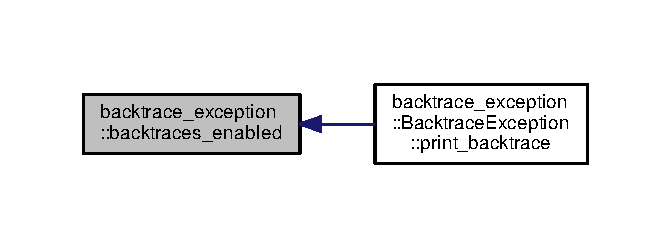
\includegraphics[width=346pt]{namespacebacktrace__exception_a68f7b8565eefc4f9b862c25ec47ce2b7_icgraph}
\end{center}
\end{figure}


\index{backtrace\+\_\+exception@{backtrace\+\_\+exception}!disable\+\_\+backtraces@{disable\+\_\+backtraces}}
\index{disable\+\_\+backtraces@{disable\+\_\+backtraces}!backtrace\+\_\+exception@{backtrace\+\_\+exception}}
\paragraph[{\texorpdfstring{disable\+\_\+backtraces()}{disable_backtraces()}}]{\setlength{\rightskip}{0pt plus 5cm}void backtrace\+\_\+exception\+::disable\+\_\+backtraces (
\begin{DoxyParamCaption}
{}
\end{DoxyParamCaption}
)}\hypertarget{namespacebacktrace__exception_a134895cbad5bc441a941f1f49b43a78a}{}\label{namespacebacktrace__exception_a134895cbad5bc441a941f1f49b43a78a}


Definition at line 74 of file Backtrace\+Exception.\+cpp.

\index{backtrace\+\_\+exception@{backtrace\+\_\+exception}!enable\+\_\+backtraces@{enable\+\_\+backtraces}}
\index{enable\+\_\+backtraces@{enable\+\_\+backtraces}!backtrace\+\_\+exception@{backtrace\+\_\+exception}}
\paragraph[{\texorpdfstring{enable\+\_\+backtraces()}{enable_backtraces()}}]{\setlength{\rightskip}{0pt plus 5cm}void backtrace\+\_\+exception\+::enable\+\_\+backtraces (
\begin{DoxyParamCaption}
{}
\end{DoxyParamCaption}
)}\hypertarget{namespacebacktrace__exception_a4e1b86dea1b116c7bac88d89448a808e}{}\label{namespacebacktrace__exception_a4e1b86dea1b116c7bac88d89448a808e}


Definition at line 79 of file Backtrace\+Exception.\+cpp.

\index{backtrace\+\_\+exception@{backtrace\+\_\+exception}!get\+\_\+backtrace\+\_\+method@{get\+\_\+backtrace\+\_\+method}}
\index{get\+\_\+backtrace\+\_\+method@{get\+\_\+backtrace\+\_\+method}!backtrace\+\_\+exception@{backtrace\+\_\+exception}}
\paragraph[{\texorpdfstring{get\+\_\+backtrace\+\_\+method()}{get_backtrace_method()}}]{\setlength{\rightskip}{0pt plus 5cm}{\bf Backtrace\+Method} backtrace\+\_\+exception\+::get\+\_\+backtrace\+\_\+method (
\begin{DoxyParamCaption}
{}
\end{DoxyParamCaption}
)}\hypertarget{namespacebacktrace__exception_a024cd6e7707e7f7cbb9283e60907142c}{}\label{namespacebacktrace__exception_a024cd6e7707e7f7cbb9283e60907142c}


Definition at line 46 of file Backtrace\+Exception.\+cpp.

\index{backtrace\+\_\+exception@{backtrace\+\_\+exception}!set\+\_\+backtrace\+\_\+method@{set\+\_\+backtrace\+\_\+method}}
\index{set\+\_\+backtrace\+\_\+method@{set\+\_\+backtrace\+\_\+method}!backtrace\+\_\+exception@{backtrace\+\_\+exception}}
\paragraph[{\texorpdfstring{set\+\_\+backtrace\+\_\+method(\+Backtrace\+Method method)}{set_backtrace_method(BacktraceMethod method)}}]{\setlength{\rightskip}{0pt plus 5cm}void backtrace\+\_\+exception\+::set\+\_\+backtrace\+\_\+method (
\begin{DoxyParamCaption}
\item[{{\bf Backtrace\+Method}}]{method}
\end{DoxyParamCaption}
)}\hypertarget{namespacebacktrace__exception_afe7dd97c0deefd1a0e9cb08f9c8089b2}{}\label{namespacebacktrace__exception_afe7dd97c0deefd1a0e9cb08f9c8089b2}


Definition at line 51 of file Backtrace\+Exception.\+cpp.



References gdb, glibc, and stackwalk.


\section{Class Documentation}
\hypertarget{classbacktrace__exception_1_1BacktraceException}{}\subsection{backtrace\+\_\+exception\+:\+:Backtrace\+Exception Class Reference}
\label{classbacktrace__exception_1_1BacktraceException}\index{backtrace\+\_\+exception\+::\+Backtrace\+Exception@{backtrace\+\_\+exception\+::\+Backtrace\+Exception}}


Extension of std\+::exception that produces saved backtraces for debugging.  




{\ttfamily \#include $<$/home/travis/build/markjolah/\+Backtrace\+Exception/include/\+Backtrace\+Exception/\+Backtrace\+Exception.\+h$>$}



Inheritance diagram for backtrace\+\_\+exception\+:\+:Backtrace\+Exception\+:\nopagebreak
\begin{figure}[H]
\begin{center}
\leavevmode
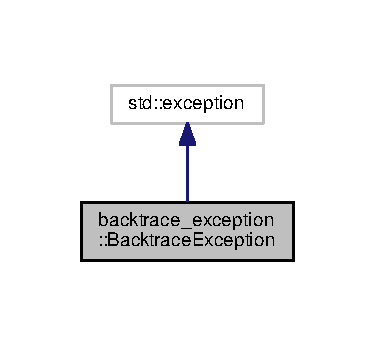
\includegraphics[width=182pt]{classbacktrace__exception_1_1BacktraceException__inherit__graph}
\end{center}
\end{figure}


Collaboration diagram for backtrace\+\_\+exception\+:\+:Backtrace\+Exception\+:\nopagebreak
\begin{figure}[H]
\begin{center}
\leavevmode
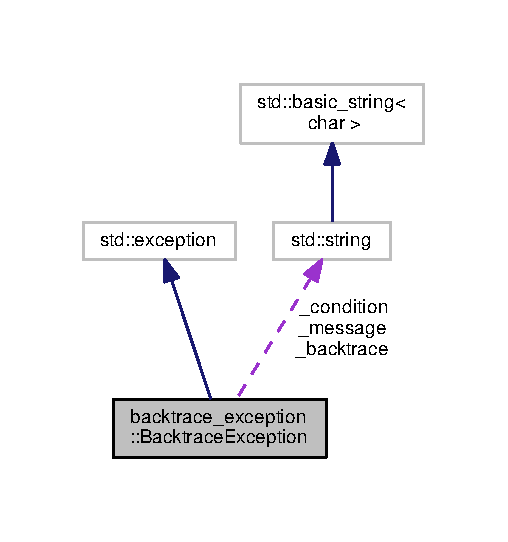
\includegraphics[width=244pt]{classbacktrace__exception_1_1BacktraceException__coll__graph}
\end{center}
\end{figure}
\subsubsection*{Public Member Functions}
\begin{DoxyCompactItemize}
\item 
\hyperlink{classbacktrace__exception_1_1BacktraceException_aa58cdade30cd7c6d60536e1f8d154fe0}{Backtrace\+Exception} (std\+::string \hyperlink{classbacktrace__exception_1_1BacktraceException_a35a4e3e649e4cbdcac45e5c6e0c9a8ec}{message})
\item 
\hyperlink{classbacktrace__exception_1_1BacktraceException_a7487e7b51e59aaae9a5cf0c9e5dc2498}{Backtrace\+Exception} (std\+::string \hyperlink{classbacktrace__exception_1_1BacktraceException_accccd52bdfdbb1ffca58a695dace84f2}{condition}, std\+::string \hyperlink{classbacktrace__exception_1_1BacktraceException_a35a4e3e649e4cbdcac45e5c6e0c9a8ec}{message})
\begin{DoxyCompactList}\small\item\em Create a \hyperlink{classbacktrace__exception_1_1BacktraceException}{Backtrace\+Exception} with specified condition. \end{DoxyCompactList}\item 
virtual const char $\ast$ \hyperlink{classbacktrace__exception_1_1BacktraceException_accccd52bdfdbb1ffca58a695dace84f2}{condition} () const noexcept
\item 
virtual const char $\ast$ \hyperlink{classbacktrace__exception_1_1BacktraceException_a35a4e3e649e4cbdcac45e5c6e0c9a8ec}{message} () const noexcept
\item 
virtual const char $\ast$ \hyperlink{classbacktrace__exception_1_1BacktraceException_a7454505fabaa8d6ef8396049f7d4e775}{backtrace} () const noexcept
\item 
const char $\ast$ \hyperlink{classbacktrace__exception_1_1BacktraceException_a865bf08728344df9ed42bb5f6aef048f}{what} () const noexceptoverride
\end{DoxyCompactItemize}
\subsubsection*{Static Public Member Functions}
\begin{DoxyCompactItemize}
\item 
static std\+::string \hyperlink{classbacktrace__exception_1_1BacktraceException_aef24b0571ea422191026a2292947810a}{print\+\_\+backtrace} ()
\end{DoxyCompactItemize}
\subsubsection*{Protected Attributes}
\begin{DoxyCompactItemize}
\item 
std\+::string \hyperlink{classbacktrace__exception_1_1BacktraceException_a3e43ec7625a2390fdfad8fffd4ab126c}{\+\_\+condition}
\item 
std\+::string \hyperlink{classbacktrace__exception_1_1BacktraceException_a34f27c079bfdf70ceb66875f3bb7d599}{\+\_\+message}
\item 
std\+::string \hyperlink{classbacktrace__exception_1_1BacktraceException_a86f9233184b7611b08faaf19b9490f43}{\+\_\+backtrace}
\end{DoxyCompactItemize}


\subsubsection{Detailed Description}
Extension of std\+::exception that produces saved backtraces for debugging. 



Definition at line 28 of file Backtrace\+Exception.\+h.



\subsubsection{Constructor \& Destructor Documentation}
\index{backtrace\+\_\+exception\+::\+Backtrace\+Exception@{backtrace\+\_\+exception\+::\+Backtrace\+Exception}!Backtrace\+Exception@{Backtrace\+Exception}}
\index{Backtrace\+Exception@{Backtrace\+Exception}!backtrace\+\_\+exception\+::\+Backtrace\+Exception@{backtrace\+\_\+exception\+::\+Backtrace\+Exception}}
\paragraph[{\texorpdfstring{Backtrace\+Exception(std\+::string message)}{BacktraceException(std::string message)}}]{\setlength{\rightskip}{0pt plus 5cm}backtrace\+\_\+exception\+::\+Backtrace\+Exception\+::\+Backtrace\+Exception (
\begin{DoxyParamCaption}
\item[{std\+::string}]{message}
\end{DoxyParamCaption}
)}\hypertarget{classbacktrace__exception_1_1BacktraceException_aa58cdade30cd7c6d60536e1f8d154fe0}{}\label{classbacktrace__exception_1_1BacktraceException_aa58cdade30cd7c6d60536e1f8d154fe0}


Definition at line 195 of file Backtrace\+Exception.\+cpp.

\index{backtrace\+\_\+exception\+::\+Backtrace\+Exception@{backtrace\+\_\+exception\+::\+Backtrace\+Exception}!Backtrace\+Exception@{Backtrace\+Exception}}
\index{Backtrace\+Exception@{Backtrace\+Exception}!backtrace\+\_\+exception\+::\+Backtrace\+Exception@{backtrace\+\_\+exception\+::\+Backtrace\+Exception}}
\paragraph[{\texorpdfstring{Backtrace\+Exception(std\+::string condition, std\+::string message)}{BacktraceException(std::string condition, std::string message)}}]{\setlength{\rightskip}{0pt plus 5cm}backtrace\+\_\+exception\+::\+Backtrace\+Exception\+::\+Backtrace\+Exception (
\begin{DoxyParamCaption}
\item[{std\+::string}]{condition, }
\item[{std\+::string}]{message}
\end{DoxyParamCaption}
)}\hypertarget{classbacktrace__exception_1_1BacktraceException_a7487e7b51e59aaae9a5cf0c9e5dc2498}{}\label{classbacktrace__exception_1_1BacktraceException_a7487e7b51e59aaae9a5cf0c9e5dc2498}


Create a \hyperlink{classbacktrace__exception_1_1BacktraceException}{Backtrace\+Exception} with specified condition. 


\begin{DoxyParams}{Parameters}
{\em condition} & A string classifying the error condition \\
\hline
{\em message} & A message string describing the error condition. \\
\hline
\end{DoxyParams}


Definition at line 199 of file Backtrace\+Exception.\+cpp.



\subsubsection{Member Function Documentation}
\index{backtrace\+\_\+exception\+::\+Backtrace\+Exception@{backtrace\+\_\+exception\+::\+Backtrace\+Exception}!backtrace@{backtrace}}
\index{backtrace@{backtrace}!backtrace\+\_\+exception\+::\+Backtrace\+Exception@{backtrace\+\_\+exception\+::\+Backtrace\+Exception}}
\paragraph[{\texorpdfstring{backtrace() const noexcept}{backtrace() const noexcept}}]{\setlength{\rightskip}{0pt plus 5cm}const char $\ast$ backtrace\+\_\+exception\+::\+Backtrace\+Exception\+::backtrace (
\begin{DoxyParamCaption}
{}
\end{DoxyParamCaption}
) const\hspace{0.3cm}{\ttfamily [inline]}, {\ttfamily [virtual]}, {\ttfamily [noexcept]}}\hypertarget{classbacktrace__exception_1_1BacktraceException_a7454505fabaa8d6ef8396049f7d4e775}{}\label{classbacktrace__exception_1_1BacktraceException_a7454505fabaa8d6ef8396049f7d4e775}


Definition at line 59 of file Backtrace\+Exception.\+h.

\index{backtrace\+\_\+exception\+::\+Backtrace\+Exception@{backtrace\+\_\+exception\+::\+Backtrace\+Exception}!condition@{condition}}
\index{condition@{condition}!backtrace\+\_\+exception\+::\+Backtrace\+Exception@{backtrace\+\_\+exception\+::\+Backtrace\+Exception}}
\paragraph[{\texorpdfstring{condition() const noexcept}{condition() const noexcept}}]{\setlength{\rightskip}{0pt plus 5cm}const char $\ast$ backtrace\+\_\+exception\+::\+Backtrace\+Exception\+::condition (
\begin{DoxyParamCaption}
{}
\end{DoxyParamCaption}
) const\hspace{0.3cm}{\ttfamily [inline]}, {\ttfamily [virtual]}, {\ttfamily [noexcept]}}\hypertarget{classbacktrace__exception_1_1BacktraceException_accccd52bdfdbb1ffca58a695dace84f2}{}\label{classbacktrace__exception_1_1BacktraceException_accccd52bdfdbb1ffca58a695dace84f2}


Definition at line 51 of file Backtrace\+Exception.\+h.

\index{backtrace\+\_\+exception\+::\+Backtrace\+Exception@{backtrace\+\_\+exception\+::\+Backtrace\+Exception}!message@{message}}
\index{message@{message}!backtrace\+\_\+exception\+::\+Backtrace\+Exception@{backtrace\+\_\+exception\+::\+Backtrace\+Exception}}
\paragraph[{\texorpdfstring{message() const noexcept}{message() const noexcept}}]{\setlength{\rightskip}{0pt plus 5cm}const char $\ast$ backtrace\+\_\+exception\+::\+Backtrace\+Exception\+::message (
\begin{DoxyParamCaption}
{}
\end{DoxyParamCaption}
) const\hspace{0.3cm}{\ttfamily [inline]}, {\ttfamily [virtual]}, {\ttfamily [noexcept]}}\hypertarget{classbacktrace__exception_1_1BacktraceException_a35a4e3e649e4cbdcac45e5c6e0c9a8ec}{}\label{classbacktrace__exception_1_1BacktraceException_a35a4e3e649e4cbdcac45e5c6e0c9a8ec}


Definition at line 55 of file Backtrace\+Exception.\+h.

\index{backtrace\+\_\+exception\+::\+Backtrace\+Exception@{backtrace\+\_\+exception\+::\+Backtrace\+Exception}!print\+\_\+backtrace@{print\+\_\+backtrace}}
\index{print\+\_\+backtrace@{print\+\_\+backtrace}!backtrace\+\_\+exception\+::\+Backtrace\+Exception@{backtrace\+\_\+exception\+::\+Backtrace\+Exception}}
\paragraph[{\texorpdfstring{print\+\_\+backtrace()}{print_backtrace()}}]{\setlength{\rightskip}{0pt plus 5cm}std\+::string backtrace\+\_\+exception\+::\+Backtrace\+Exception\+::print\+\_\+backtrace (
\begin{DoxyParamCaption}
{}
\end{DoxyParamCaption}
)\hspace{0.3cm}{\ttfamily [static]}}\hypertarget{classbacktrace__exception_1_1BacktraceException_aef24b0571ea422191026a2292947810a}{}\label{classbacktrace__exception_1_1BacktraceException_aef24b0571ea422191026a2292947810a}


Definition at line 211 of file Backtrace\+Exception.\+cpp.



References backtrace\+\_\+exception\+::backtraces\+\_\+enabled(), backtrace\+\_\+exception\+::gdb, and backtrace\+\_\+exception\+::glibc.



Here is the call graph for this function\+:\nopagebreak
\begin{figure}[H]
\begin{center}
\leavevmode
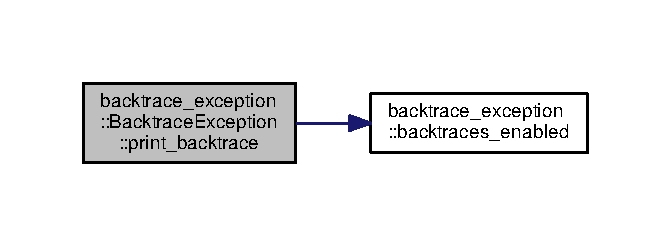
\includegraphics[width=322pt]{classbacktrace__exception_1_1BacktraceException_aef24b0571ea422191026a2292947810a_cgraph}
\end{center}
\end{figure}


\index{backtrace\+\_\+exception\+::\+Backtrace\+Exception@{backtrace\+\_\+exception\+::\+Backtrace\+Exception}!what@{what}}
\index{what@{what}!backtrace\+\_\+exception\+::\+Backtrace\+Exception@{backtrace\+\_\+exception\+::\+Backtrace\+Exception}}
\paragraph[{\texorpdfstring{what() const noexceptoverride}{what() const noexceptoverride}}]{\setlength{\rightskip}{0pt plus 5cm}const char $\ast$ backtrace\+\_\+exception\+::\+Backtrace\+Exception\+::what (
\begin{DoxyParamCaption}
{}
\end{DoxyParamCaption}
) const\hspace{0.3cm}{\ttfamily [override]}, {\ttfamily [noexcept]}}\hypertarget{classbacktrace__exception_1_1BacktraceException_a865bf08728344df9ed42bb5f6aef048f}{}\label{classbacktrace__exception_1_1BacktraceException_a865bf08728344df9ed42bb5f6aef048f}


Definition at line 203 of file Backtrace\+Exception.\+cpp.



References \+\_\+backtrace, \+\_\+condition, \+\_\+message, and backtrace\+\_\+exception\+::backtraces\+\_\+enabled().



Here is the call graph for this function\+:\nopagebreak
\begin{figure}[H]
\begin{center}
\leavevmode
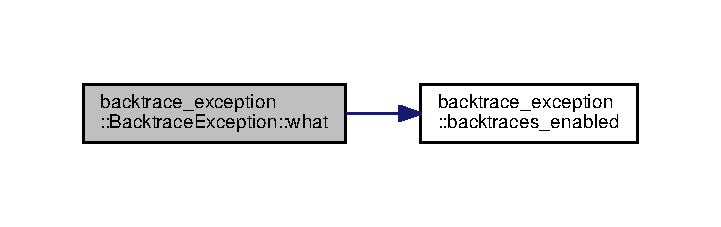
\includegraphics[width=346pt]{classbacktrace__exception_1_1BacktraceException_a865bf08728344df9ed42bb5f6aef048f_cgraph}
\end{center}
\end{figure}




\subsubsection{Member Data Documentation}
\index{backtrace\+\_\+exception\+::\+Backtrace\+Exception@{backtrace\+\_\+exception\+::\+Backtrace\+Exception}!\+\_\+backtrace@{\+\_\+backtrace}}
\index{\+\_\+backtrace@{\+\_\+backtrace}!backtrace\+\_\+exception\+::\+Backtrace\+Exception@{backtrace\+\_\+exception\+::\+Backtrace\+Exception}}
\paragraph[{\texorpdfstring{\+\_\+backtrace}{_backtrace}}]{\setlength{\rightskip}{0pt plus 5cm}std\+::string backtrace\+\_\+exception\+::\+Backtrace\+Exception\+::\+\_\+backtrace\hspace{0.3cm}{\ttfamily [protected]}}\hypertarget{classbacktrace__exception_1_1BacktraceException_a86f9233184b7611b08faaf19b9490f43}{}\label{classbacktrace__exception_1_1BacktraceException_a86f9233184b7611b08faaf19b9490f43}


Definition at line 47 of file Backtrace\+Exception.\+h.



Referenced by what().

\index{backtrace\+\_\+exception\+::\+Backtrace\+Exception@{backtrace\+\_\+exception\+::\+Backtrace\+Exception}!\+\_\+condition@{\+\_\+condition}}
\index{\+\_\+condition@{\+\_\+condition}!backtrace\+\_\+exception\+::\+Backtrace\+Exception@{backtrace\+\_\+exception\+::\+Backtrace\+Exception}}
\paragraph[{\texorpdfstring{\+\_\+condition}{_condition}}]{\setlength{\rightskip}{0pt plus 5cm}std\+::string backtrace\+\_\+exception\+::\+Backtrace\+Exception\+::\+\_\+condition\hspace{0.3cm}{\ttfamily [protected]}}\hypertarget{classbacktrace__exception_1_1BacktraceException_a3e43ec7625a2390fdfad8fffd4ab126c}{}\label{classbacktrace__exception_1_1BacktraceException_a3e43ec7625a2390fdfad8fffd4ab126c}


Definition at line 45 of file Backtrace\+Exception.\+h.



Referenced by what().

\index{backtrace\+\_\+exception\+::\+Backtrace\+Exception@{backtrace\+\_\+exception\+::\+Backtrace\+Exception}!\+\_\+message@{\+\_\+message}}
\index{\+\_\+message@{\+\_\+message}!backtrace\+\_\+exception\+::\+Backtrace\+Exception@{backtrace\+\_\+exception\+::\+Backtrace\+Exception}}
\paragraph[{\texorpdfstring{\+\_\+message}{_message}}]{\setlength{\rightskip}{0pt plus 5cm}std\+::string backtrace\+\_\+exception\+::\+Backtrace\+Exception\+::\+\_\+message\hspace{0.3cm}{\ttfamily [protected]}}\hypertarget{classbacktrace__exception_1_1BacktraceException_a34f27c079bfdf70ceb66875f3bb7d599}{}\label{classbacktrace__exception_1_1BacktraceException_a34f27c079bfdf70ceb66875f3bb7d599}


Definition at line 46 of file Backtrace\+Exception.\+h.



Referenced by what().



The documentation for this class was generated from the following files\+:\begin{DoxyCompactItemize}
\item 
\hyperlink{BacktraceException_8h}{Backtrace\+Exception.\+h}\item 
\hyperlink{BacktraceException_8cpp}{Backtrace\+Exception.\+cpp}\end{DoxyCompactItemize}

\section{File Documentation}
\hypertarget{BacktraceException_8cpp}{\subsection{Backtrace\-Exception.\-cpp File Reference}
\label{BacktraceException_8cpp}\index{Backtrace\-Exception.\-cpp@{Backtrace\-Exception.\-cpp}}
}


Backtrace\-Exception class member function definitions.  


{\ttfamily \#include \char`\"{}Backtrace\-Exception/\-Backtrace\-Exception.\-h\char`\"{}}\\*
{\ttfamily \#include $<$cstdlib$>$}\\*
{\ttfamily \#include $<$memory$>$}\\*
{\ttfamily \#include $<$iostream$>$}\\*
{\ttfamily \#include $<$string$>$}\\*
{\ttfamily \#include $<$sstream$>$}\\*
{\ttfamily \#include $<$vector$>$}\\*
Include dependency graph for Backtrace\-Exception.\-cpp\-:\nopagebreak
\begin{figure}[H]
\begin{center}
\leavevmode
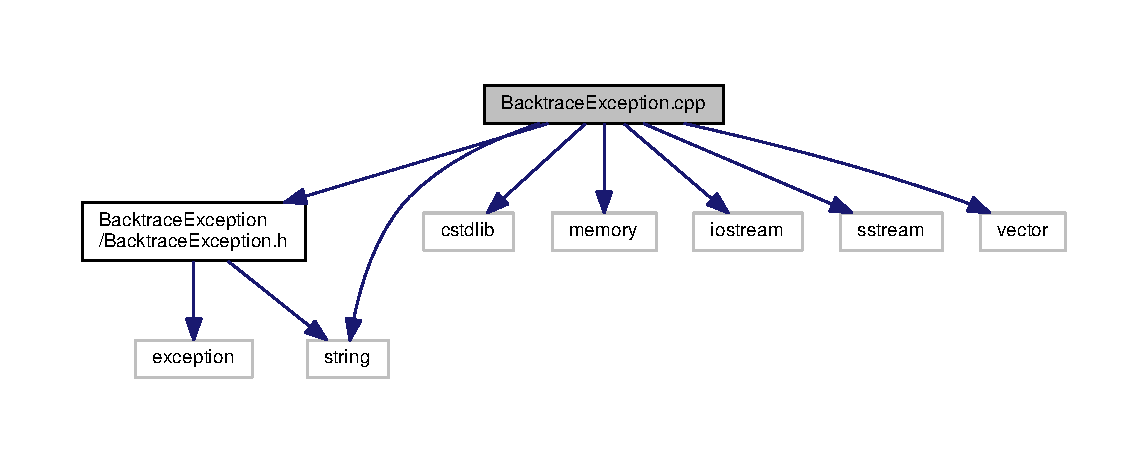
\includegraphics[width=350pt]{BacktraceException_8cpp__incl}
\end{center}
\end{figure}
\subsubsection*{Namespaces}
\begin{DoxyCompactItemize}
\item 
\hyperlink{namespacebacktrace__exception}{backtrace\-\_\-exception}
\end{DoxyCompactItemize}
\subsubsection*{Functions}
\begin{DoxyCompactItemize}
\item 
Backtrace\-Method \hyperlink{namespacebacktrace__exception_a024cd6e7707e7f7cbb9283e60907142c}{backtrace\-\_\-exception\-::get\-\_\-backtrace\-\_\-method} ()
\item 
void \hyperlink{namespacebacktrace__exception_afe7dd97c0deefd1a0e9cb08f9c8089b2}{backtrace\-\_\-exception\-::set\-\_\-backtrace\-\_\-method} (Backtrace\-Method method)
\item 
void \hyperlink{namespacebacktrace__exception_a134895cbad5bc441a941f1f49b43a78a}{backtrace\-\_\-exception\-::disable\-\_\-backtraces} ()
\item 
void \hyperlink{namespacebacktrace__exception_a4e1b86dea1b116c7bac88d89448a808e}{backtrace\-\_\-exception\-::enable\-\_\-backtraces} ()
\item 
bool \hyperlink{namespacebacktrace__exception_a68f7b8565eefc4f9b862c25ec47ce2b7}{backtrace\-\_\-exception\-::backtraces\-\_\-enabled} ()
\end{DoxyCompactItemize}


\subsubsection{Detailed Description}
Backtrace\-Exception class member function definitions. \begin{DoxyAuthor}{Author}
Mark J. Olah (mjo@cs.\-unm D\-O\-T edu) 
\end{DoxyAuthor}
\begin{DoxyDate}{Date}
2017 -\/ 2018 
\end{DoxyDate}
\begin{DoxyCopyright}{Copyright}
Licensed under the Apache License, Version 2.\-0. See L\-I\-C\-E\-N\-S\-E file. 
\end{DoxyCopyright}


Definition in file \hyperlink{BacktraceException_8cpp_source}{Backtrace\-Exception.\-cpp}.


\hypertarget{BacktraceException_8h}{\subsection{Backtrace\-Exception.\-h File Reference}
\label{BacktraceException_8h}\index{Backtrace\-Exception.\-h@{Backtrace\-Exception.\-h}}
}


Backtrace\-Exception class declaration and inline member functions.  


{\ttfamily \#include $<$exception$>$}\\*
{\ttfamily \#include $<$string$>$}\\*
Include dependency graph for Backtrace\-Exception.\-h\-:\nopagebreak
\begin{figure}[H]
\begin{center}
\leavevmode
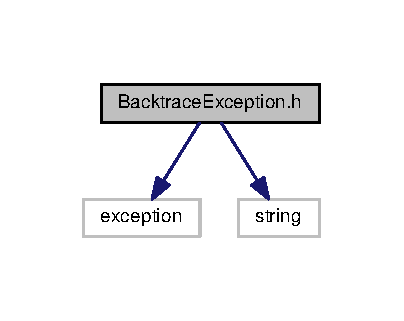
\includegraphics[width=193pt]{BacktraceException_8h__incl}
\end{center}
\end{figure}
This graph shows which files directly or indirectly include this file\-:\nopagebreak
\begin{figure}[H]
\begin{center}
\leavevmode
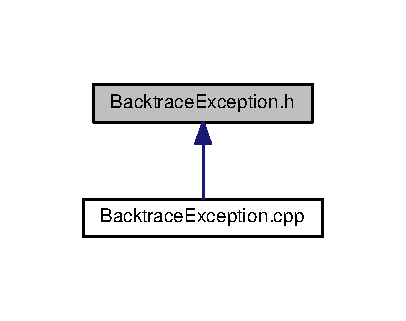
\includegraphics[width=194pt]{BacktraceException_8h__dep__incl}
\end{center}
\end{figure}
\subsubsection*{Classes}
\begin{DoxyCompactItemize}
\item 
class \hyperlink{classbacktrace__exception_1_1BacktraceException}{backtrace\-\_\-exception\-::\-Backtrace\-Exception}
\begin{DoxyCompactList}\small\item\em Extension of std\-::exception that produces saved backtraces for debugging. \end{DoxyCompactList}\end{DoxyCompactItemize}
\subsubsection*{Namespaces}
\begin{DoxyCompactItemize}
\item 
\hyperlink{namespacebacktrace__exception}{backtrace\-\_\-exception}
\end{DoxyCompactItemize}
\subsubsection*{Enumerations}
\begin{DoxyCompactItemize}
\item 
enum \hyperlink{namespacebacktrace__exception_ac04b358e6d3eac08b792a7c2e99b57cc}{backtrace\-\_\-exception\-::\-Backtrace\-Method} \{ \hyperlink{namespacebacktrace__exception_ac04b358e6d3eac08b792a7c2e99b57cca0ded6244fb02e7fb8db8e873d25656c5}{backtrace\-\_\-exception\-::\-Backtrace\-Method\-::glibc}, 
\hyperlink{namespacebacktrace__exception_ac04b358e6d3eac08b792a7c2e99b57ccaca3e1c20efd5690f9789a87c66a5047a}{backtrace\-\_\-exception\-::\-Backtrace\-Method\-::gdb}, 
\hyperlink{namespacebacktrace__exception_ac04b358e6d3eac08b792a7c2e99b57ccac87739aef758816341a559291c49bbbb}{backtrace\-\_\-exception\-::\-Backtrace\-Method\-::stackwalk}
 \}
\end{DoxyCompactItemize}
\subsubsection*{Functions}
\begin{DoxyCompactItemize}
\item 
void \hyperlink{namespacebacktrace__exception_a134895cbad5bc441a941f1f49b43a78a}{backtrace\-\_\-exception\-::disable\-\_\-backtraces} ()
\item 
void \hyperlink{namespacebacktrace__exception_a4e1b86dea1b116c7bac88d89448a808e}{backtrace\-\_\-exception\-::enable\-\_\-backtraces} ()
\item 
bool \hyperlink{namespacebacktrace__exception_a68f7b8565eefc4f9b862c25ec47ce2b7}{backtrace\-\_\-exception\-::backtraces\-\_\-enabled} ()
\item 
Backtrace\-Method \hyperlink{namespacebacktrace__exception_a024cd6e7707e7f7cbb9283e60907142c}{backtrace\-\_\-exception\-::get\-\_\-backtrace\-\_\-method} ()
\item 
void \hyperlink{namespacebacktrace__exception_afe7dd97c0deefd1a0e9cb08f9c8089b2}{backtrace\-\_\-exception\-::set\-\_\-backtrace\-\_\-method} (Backtrace\-Method method)
\end{DoxyCompactItemize}


\subsubsection{Detailed Description}
Backtrace\-Exception class declaration and inline member functions. \begin{DoxyAuthor}{Author}
Mark J. Olah (mjo@cs.\-unm D\-O\-T edu) 
\end{DoxyAuthor}
\begin{DoxyDate}{Date}
2017 -\/ 2018 
\end{DoxyDate}
\begin{DoxyCopyright}{Copyright}
Licensed under the Apache License, Version 2.\-0. See L\-I\-C\-E\-N\-S\-E file. 
\end{DoxyCopyright}


Definition in file \hyperlink{BacktraceException_8h_source}{Backtrace\-Exception.\-h}.


\hypertarget{README_8md}{\subsection{R\-E\-A\-D\-M\-E.\-md File Reference}
\label{README_8md}\index{R\-E\-A\-D\-M\-E.\-md@{R\-E\-A\-D\-M\-E.\-md}}
}

%--- End generated contents ---

% Index
\newpage
\phantomsection
\clearemptydoublepage
\addcontentsline{toc}{section}{Index}
\printindex

\end{document}
